\subsection{Arduino UNO R3}

Esta tarjeta se encarga de recibir y almacenar el orden de cada señal entregada ~\cite{buitrago}. 

Es el microcontrolador principal que controla todas las funciones básicas del sistema, como leer datos de los sensores (nivel de llenado, detección de movimiento) y activar los actuadores (abrir/cerrar la tapa del cubo). También es el que recibe las señales de los sensores y ejecuta las acciones correspondientes, como encender un buzzer o enviar alertas.


\begin{figure}[htb]
	\centering
	\includegraphics[scale  = 0.50]{Imagenes/uno3.jpg}
	\caption{ARDUINO UNO R3 }{Fuente: Adaptado de~\cite{mecafenix}}

\end{figure}

\subsection{IDE Arduino}

El entorno de programaciónde la  placa  de  Arduino  se denomina Integrated  Development  Environment (IDE)el cual  permite  llevar  a  cabo  la  escritura  de  las  sentencias para el funcionamiento de los elementos físicos de la placa de Arduino. Este   software   tiene   por   si   solo   un   conjunto   de herramientas que permite,  editar  el  código,  compilar  y depurar todo a través de una interfaz gráfica, así mismo, nos    da    la    oportunidad    de    interactuar    con    el microcontrolador almacenando los programas  realizados en  su  memoria  interna  para  poner  en  marcha  todo  el hardware. El lenguaje que utiliza el IDE de Arduino está basado en C/C++ de una manera más simplificada, ofreciendo la oportunidad de cargar librerías que sean necesarias para el buen funcionamiento de nuestros proyectos ~\cite{perez}.

\begin{figure}[htb]
	\centering
	\includegraphics[scale  = 0.80]{Imagenes/ide.png}
	\caption{IDE Arduino}{Fuente: Adaptado de~\cite{perez}}

\end{figure}

\subsection{Micropython}

MicroPython es una reimplementación del lenguaje de programación Python que apunta a microcontroladores y sistemas integrados.

Los microcontroladores son computadoras compactadas en un solo chip muy pequeño. Los sistemas integrados son computadoras que funcionan dentro de un sistema mecánico o eléctrico más grande~\cite{tollervey}.

Los sistemas integrados a menudo utilizan microcontroladores.

\begin{figure}[H]
	\centering
	\includegraphics[scale  = 0.60]{Imagenes/mycro.png}
	\caption{Interfaz de MicroPython}{Fuente: Adaptado de~\cite{mpy}}
\end{figure}


\subsection{CNN}

Una red neuronal convolucional es un tipo de red neuronal artificial donde las neuronas artificiales, corresponden a campos receptivos de una manera muy similar a las neuronas en la corteza visual primaria (V1) de un cerebro biológico. Este tipo de red es una variación de un perceptron multicapa, sin embargo, debido a que su aplicación es realizada en matrices bidimensionales, son muy efectivas para tareas de visión artificial, como en la clasificación y segmentación de imágenes, entre otras aplicaciones~\cite{red_neuronal}.

\begin{figure}[htb]
	\centering
	\includegraphics[scale  = 0.80]{Imagenes/cnn.png}
	\caption{Arquitectura de una red CNN}{Fuente: Adaptado de~\cite{red_neuronal}}

\end{figure}

\subsection{Visión Artificial}

Es una disciplina científica que incluye métodos para adquirir, procesar, analizar y comprender las imágenes del mundo real con el fin de producir información numérica o simbólica para que puedan ser tratados por un ordenador. Tal y como los seres humanos usamos nuestros ojos y cerebros para comprender el mundo que nos rodea, la visión informática trata de producir el mismo efecto para que los ordenadores puedan percibir y comprender una imagen o secuencia de imágenes y actuar según convenga en una determinada situación. Esta comprensión se consigue gracias a distintos campos como la geometría, la estadística, la física y otras disciplinas. La adquisición de los datos se consigue por varios medios como secuencias de imágenes, vistas desde varias cámaras de video o datos multidimensionales desde un escáner médico~\cite{vision_artificial}.

\subsection{TensorFlow Lite}

\textbf{TensorFlow Lite}, ahora conocido como LiteRT (abreviatura de Lite Runtime), es el entorno de ejecución de alto rendimiento de Google para IA en dispositivos. Se pueden encontrar modelos LiteRT listos para ejecutar para una amplia gama de tareas de ML/IA, o convertir y ejecutar modelos TensorFlow, PyTorch y JAX al formato TFLite mediante las herramientas de conversión y optimización de AI Edge.~\cite{tensorflowlite_google}. 

Características principales:

\begin{itemize}
    \item \textbf{Optimizado para el aprendizaje automático en el dispositivo}: LiteRT aborda cinco restricciones clave de ODML: latencia (no hay viaje de ida y vuelta a un servidor), privacidad (ningún dato personal sale del dispositivo), conectividad (no se requiere conectividad a Internet), tamaño (modelo reducido y tamaño binario) y consumo de energía (inferencia eficiente y falta de conexiones de red).
    \item \textbf{Compatibilidad con múltiples plataformas}: compatible con dispositivos Android e iOS, Linux integrado y microcontroladores.
    \item \textbf{Opciones de modelos de múltiples marcos}: AI Edge proporciona herramientas para convertir modelos de TensorFlow, PyTorch y JAX al formato FlatBuffers (.tflite), lo que le permite utilizar una amplia gama de modelos de última generación en LiteRT. También tiene acceso a herramientas de optimización de modelos que pueden manejar la cuantificación y los metadatos.
    \item \textbf{Compatibilidad con diversos lenguajes}: incluye SDK para Java/Kotlin, Swift, Objective-C, C++ y Python.
    \item \textbf{Alto rendimiento}: aceleración de hardware a través de delegados especializados como GPU y iOS Core ML.
\end{itemize}

\begin{figure}[H]
	\centering
	
\includegraphics[scale  = 0.30]{Imagenes/tensorflow-lite.png}
	\caption{Logo de TensorFlow Lite}{Fuente: Adaptado de~\cite{tensorflowlite_wiki}}
\end{figure}

\subsubsection{Edge Impulse}

\textbf{Edge Impulse} es una plataforma de desarrollo de aprendizaje automático (ML) diseñada específicamente para dispositivos de computación en el borde (edge devices). Permite a los desarrolladores crear, entrenar, implementar y optimizar modelos de inteligencia artificial para dispositivos con recursos limitados, como microcontroladores, sensores y otros dispositivos IoT.~\cite{edge_impulse}

Características principales:

\begin{itemize}
    \item \textbf{Captura y preprocesamiento de datos}: Proporciona herramientas para recolectar datos desde dispositivos conectados y prepararlos para el entrenamiento de modelos.
    \item \textbf{Entrenamiento de modelos ML}: Ofrece un entorno simplificado para entrenar modelos utilizando aprendizaje supervisado o no supervisado.
    \item \textbf{Optimización para el borde}: Los modelos generados son ligeros, eficientes en energía y optimizados para ejecutarse directamente en dispositivos con hardware limitado.
    \item \textbf{Compatibilidad con hardware}: Soporta múltiples plataformas, como Arduino, Raspberry Pi, ESP32, y más.
    \item \textbf{Despliegue y análisis}: Permite implementar los modelos en dispositivos reales y analizar su rendimiento en tiempo real.
\end{itemize}

\begin{figure}[htb]
	\centering
	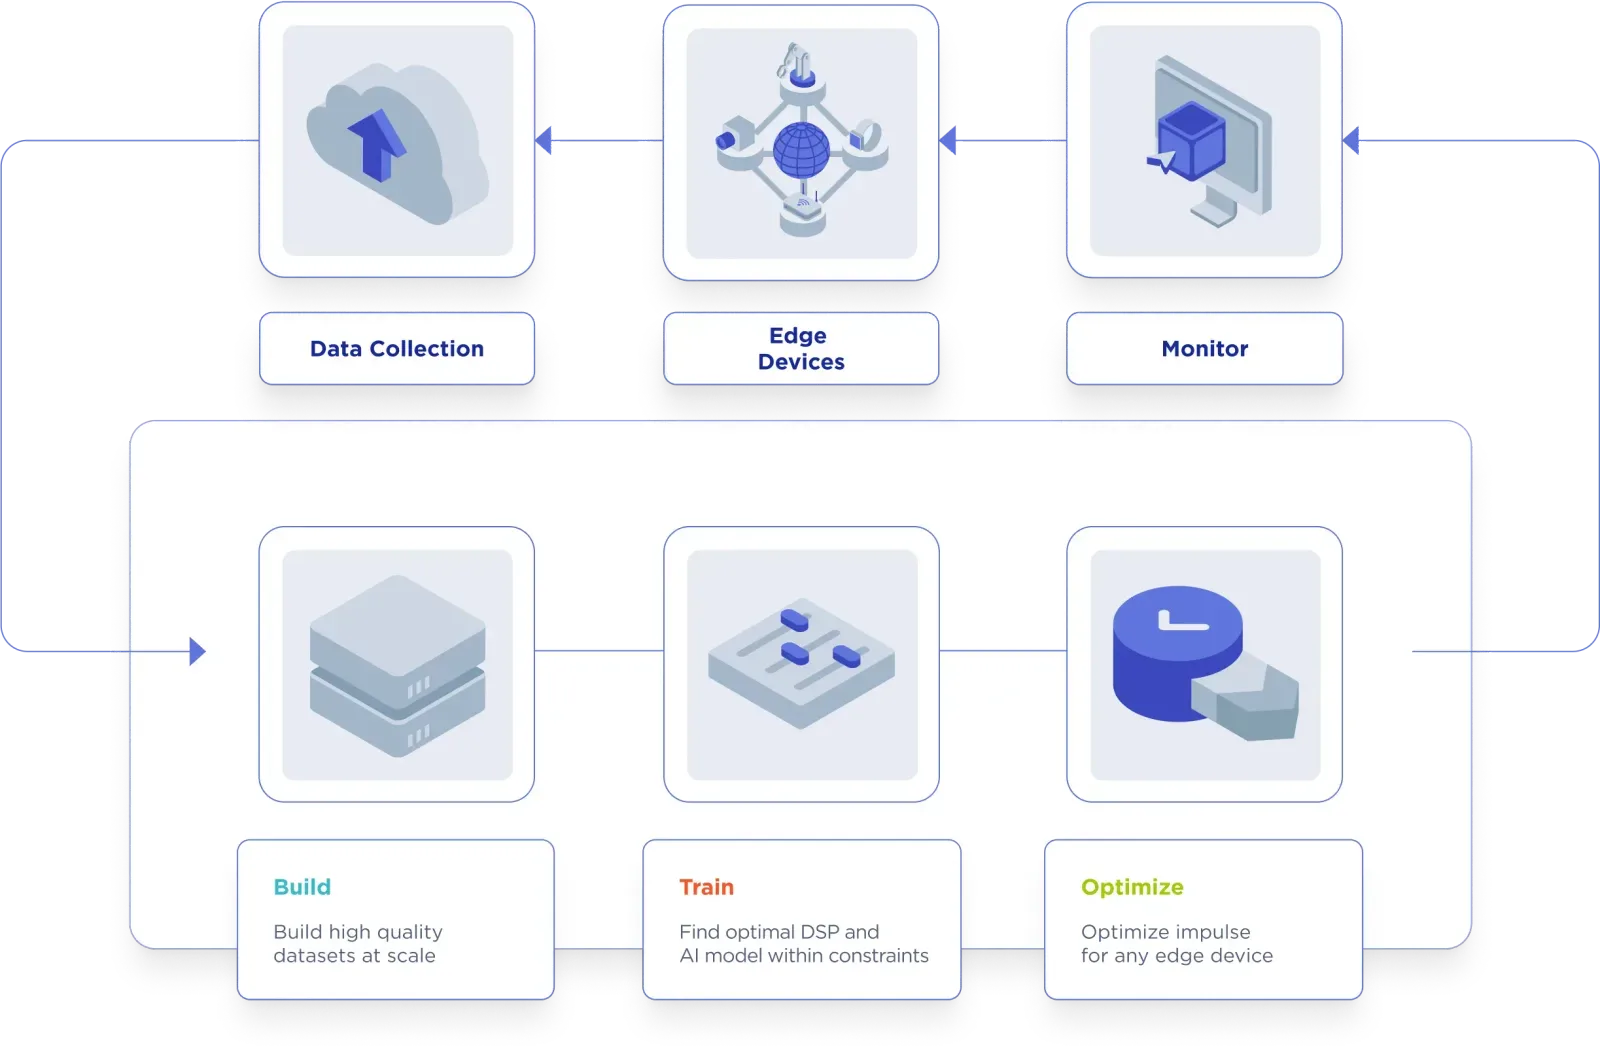
\includegraphics[scale  = 0.20]{Imagenes/edge-impulse-flujo.png}
	\caption{Flujo de trabajo de Edge Impulse}{Fuente: Adaptado de~\cite{edge_impulse}}
\end{figure}

La tecnología artificial de borde permite:

\begin{itemize}
    \item \textbf{Entornos de fabricación y operaciones}:La inteligencia artificial de borde ofrece un inmenso potencial para mitigar pérdidas financieras significativas al abordar problemas como el tiempo de inactividad de las máquinas, la ineficiencia y los problemas de control de calidad mediante la detección temprana de anomalías. La implementación de inteligencia artificial de borde en la fuente de datos mejora la seguridad, reduce la latencia y acelera la toma de decisiones para los operadores de servicios, los equipos de control de calidad y otras partes interesadas, lo que en última instancia mejora la calidad y la eficiencia.
    \item \textbf{Desarrollo de productos}:Acelera el desarrollo y aumenta drásticamente las posibilidades de implementar con éxito la inteligencia artificial de borde. Realiza iteraciones rápidas para validar ideas en una plataforma que promueva la colaboración entre equipos.
\end{itemize}

\begin{figure}[htb]
	\centering
	
\includegraphics[scale  = 0.80]{Imagenes/edge-impulse-logo.png}
	\caption{Logo de Edge Impulse}{Fuente: Adaptado de~\cite{edge_impulse}}
\end{figure}

\subsection{XIAO ESP32 CAM}
El ESP32-CAM es un módulo de cámara muy pequeño y económico que cuenta con el chip ESP32-S. Además de la cámara OV2640 y varios GPIO para conectar periféricos, también cuenta con una ranura para tarjeta microSD que puede ser útil para almacenar imágenes tomadas con la cámara o para almacenar archivos para servir a los clientes 

\begin{figure}[htb]
	\centering
	\includegraphics[scale  = 0.70]{Imagenes/xiao.png}
	\caption{XIAO ESP32 CAM}{Fuente: Adaptado de~\cite{foto_xiao}}
\end{figure}

\begin{figure}[htb]
	\centering
	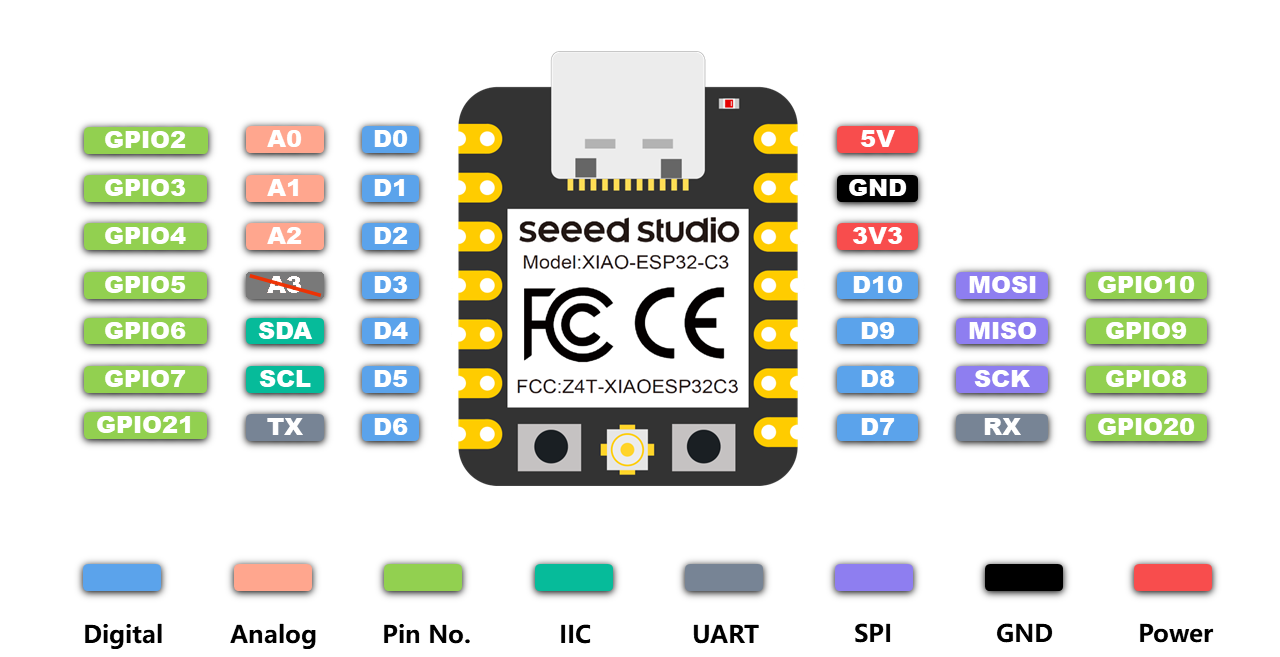
\includegraphics[scale  = 0.40]{Imagenes/diagrama_pines.png}
	\caption{Diagrama de pines}{Fuente: Adaptado de~\cite{esp32_wiki}}
\end{figure}

\begin{figure}[H]
	\centering
	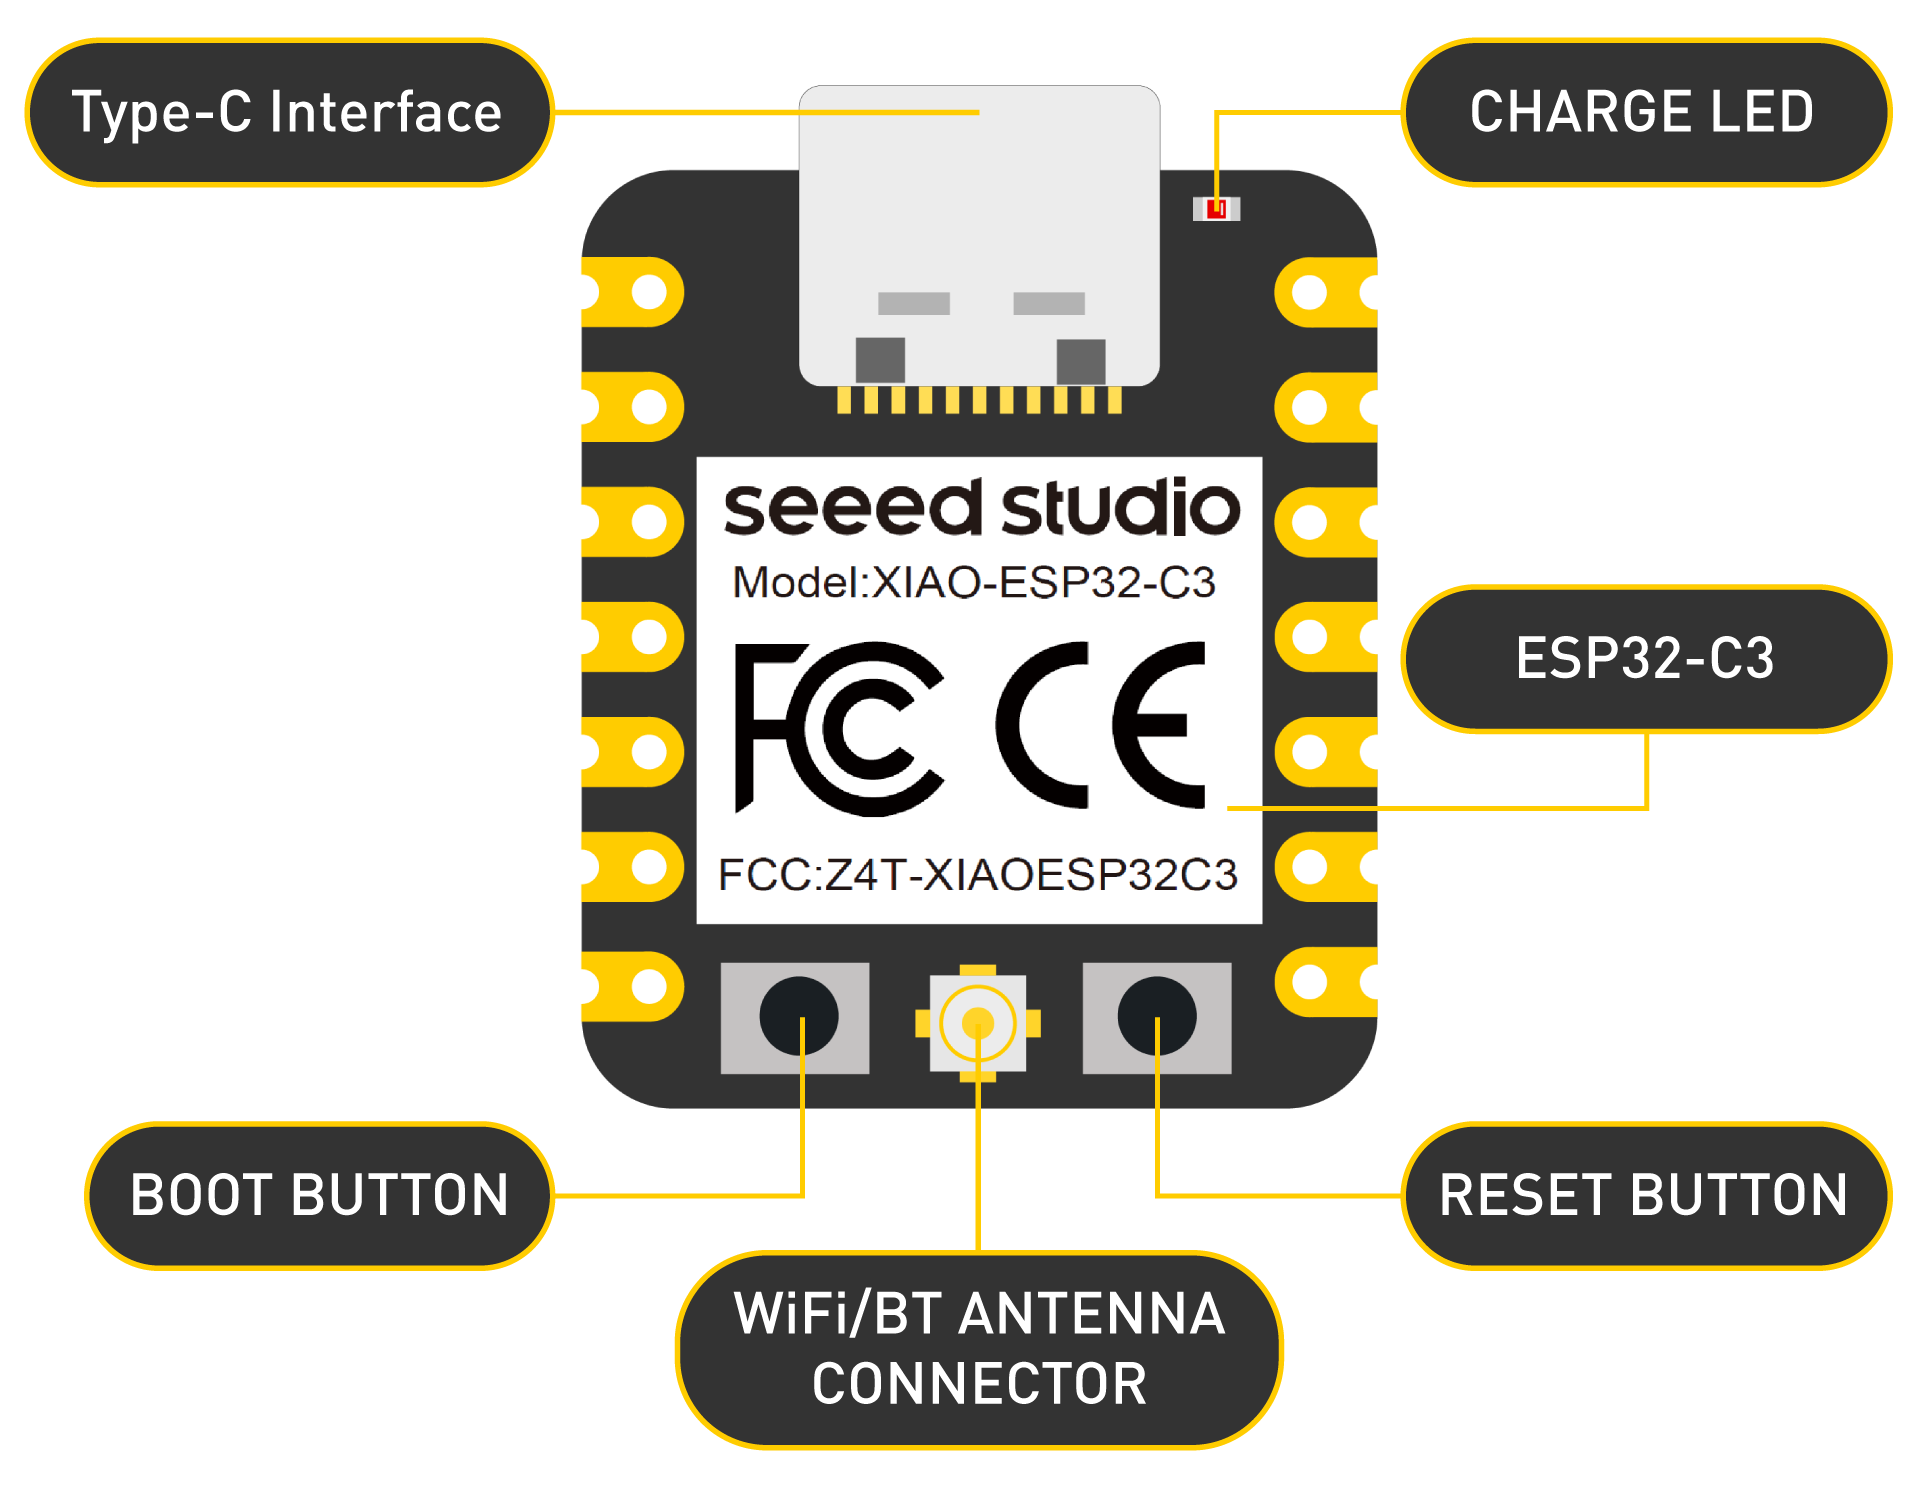
\includegraphics[scale  = 0.20]{Imagenes/parte_frontal.png}
	\caption{Componentes frontales}{Fuente: Adaptado de~\cite{esp32_wiki}}
\end{figure}

\begin{figure}[htb]
	\centering
	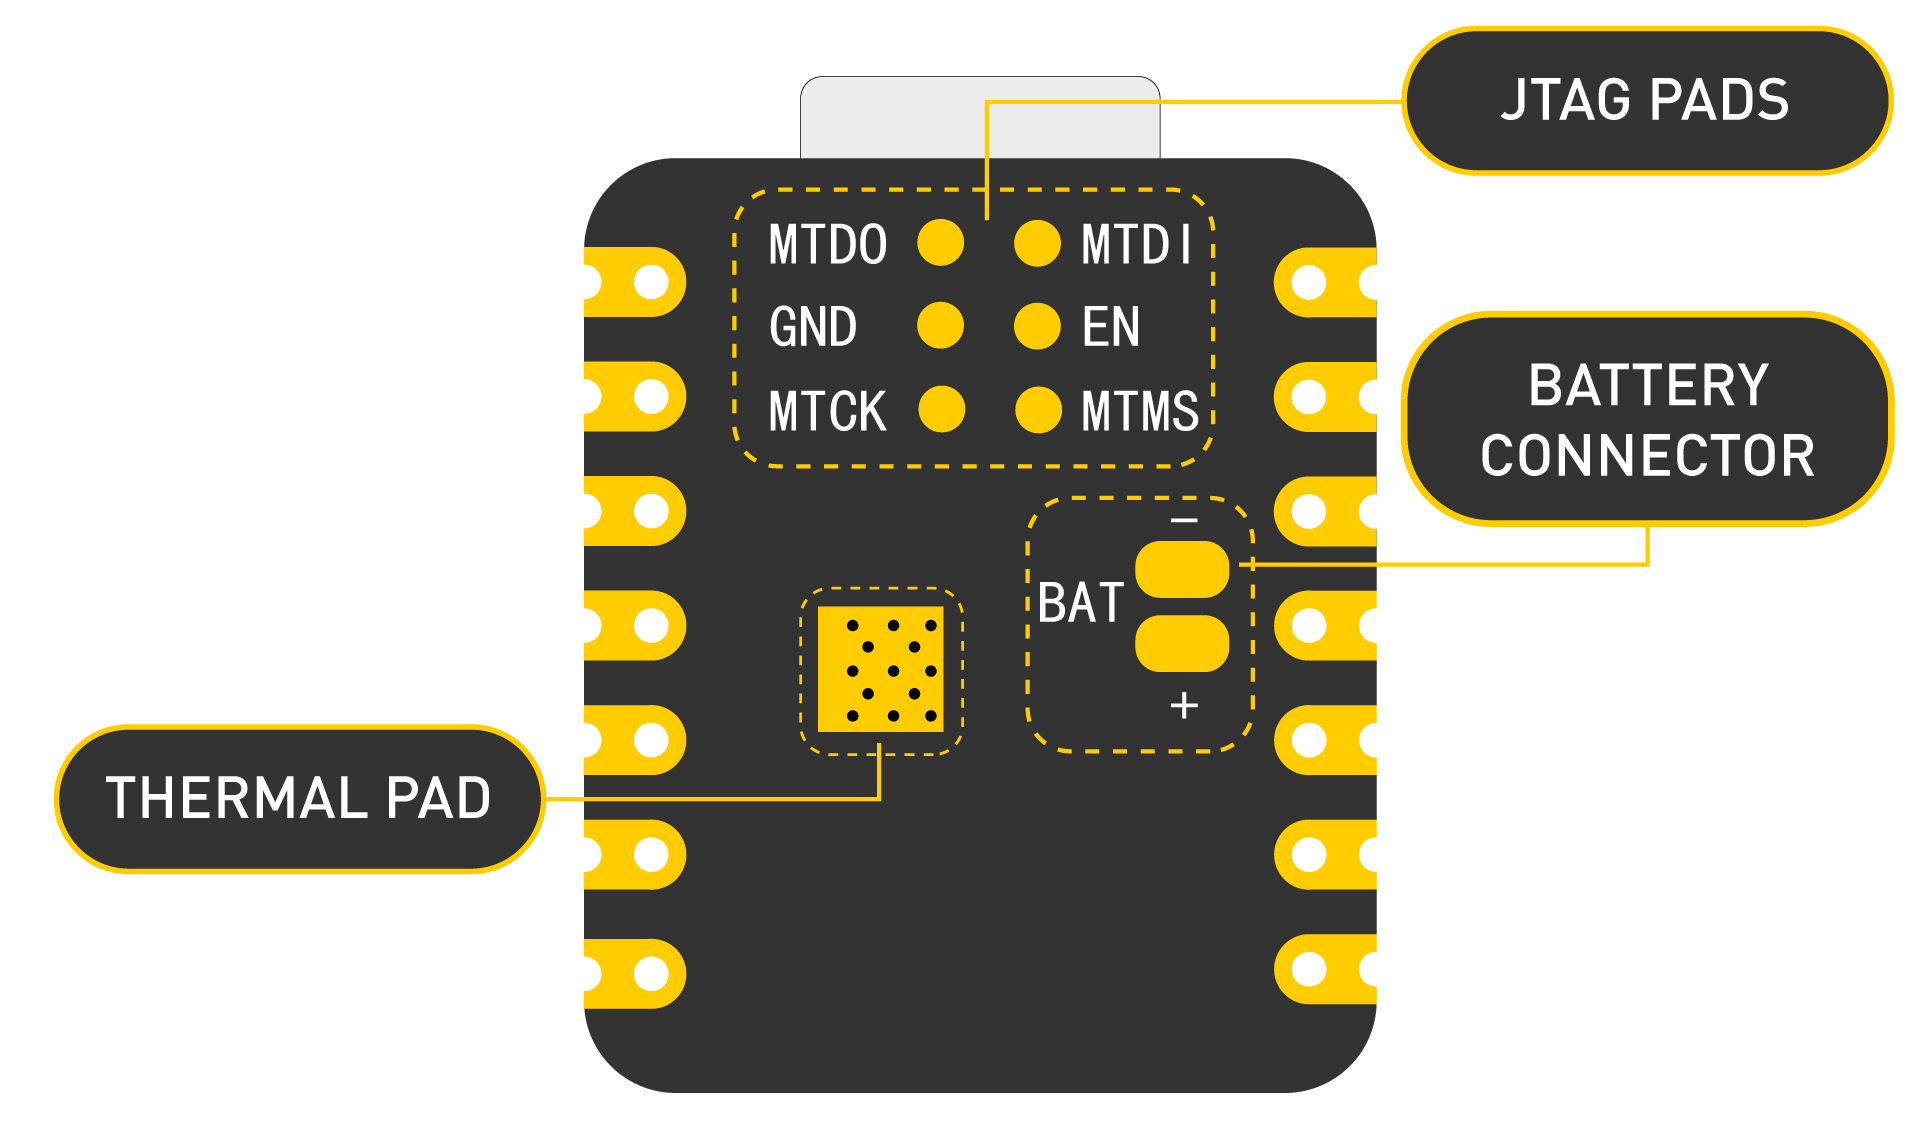
\includegraphics[scale  = 0.20]{Imagenes/parte_trasera.png}
	\caption{Componentes traseros}{Fuente: Adaptado de~\cite{esp32_wiki}}
\end{figure}

A continuación, se presenta el DataSheet encontrado.

\begin{table}[H]
    \centering
    \begin{tabularx}{\textwidth}{|l|X|} % Usar X para columnas que se expanden
        \hline
        \textbf{Ítem} & \textbf{Descripción} \\ 
        \hline
        \textbf{Procesador} & ESP32-S3R8, Xtensa LX7 de doble núcleo, 32 bits, hasta 240 MHz \\ 
        \hline
        \textbf{Inalámbrico} & Subsistema Wi-Fi completo de 2.4GHz, BLE: Bluetooth 5.0, Bluetooth mesh \\ 
        \hline
        \textbf{Sensores Integrados} & Sensor de cámara OV2640 (1600*1200), Micrófono digital \\ 
        \hline
        \textbf{Memoria} & 8M PSRAM y 8MB Flash en chip, Ranura para tarjeta SD (hasta 32GB FAT) \\ 
        \hline
        \textbf{Interfaz} & 1x UART, 1x IIC, 1x IIS, 1x SPI, 11x GPIOs (PWM), 9x ADC, 1x LED de usuario, 1x LED de carga \\ 
        & 1x conector B2B (2 GPIOs adicionales), 1x botón de reinicio, 1x botón de arranque \\ 
        \hline
        \textbf{Dimensiones} & 21 x 17.8 x 15 mm (con placa de expansión) \\ 
        \hline
        \textbf{Alimentación} & Voltaje de entrada (Type-C): 5V, Voltaje de entrada (BAT): 4.2V \\ 
        & Voltaje de operación (Type-C): 5V@38.3mA, Voltaje de operación (BAT): 3.8V@43.2mA (con expansión) \\ 
        \hline
        \textbf{Modelo de Bajo Consumo} & Sueño de módem: ~44mA, Sueño ligero: ~5mA, Sueño profundo: ~3mA \\ 
        \hline
        \textbf{Consumo de Potencia (Wi-Fi)} & Modelo activo: ~110 mA (con expansión) \\ 
        \hline
        \textbf{Consumo de Potencia (BLE)} & Modelo activo: ~102 mA (con expansión) \\ 
        \hline
        \textbf{Temperatura de Funcionamiento} & -40°C ~ 65°C \\ 
        \hline
    \end{tabularx}
    \caption{DataSheet de la XIAO ESP32 CAM}{Fuente: ~\cite{xiaotabla}}
\end{table}

\subsection{Sensor ultrasónico (HC-SR04)}

Este sensor mide la distancia entre el sensor y el nivel de basura dentro del cubo. Con esta información, se puede calcular el porcentaje de llenado. Funciona enviando pulsos ultrasónicos y midiendo el tiempo que tarda en regresar el eco, lo que indica la distancia al objeto más cercano (en este caso, la basura).

\begin{figure}[htb]
	\centering
	\includegraphics[scale  = 0.50]{Imagenes/ultra.png}
	\caption{Sensor ultrasónico HC-SR04}{Fuente: Adaptado de~\cite{ultrasonc}}

\end{figure}

\begin{table}[H]
    \centering
    \begin{tabularx}{\textwidth}{|l|X|} % Usar X para columnas que se expanden
        \hline
        \textbf{Especificación} & \textbf{Descripción} \\ 
        \hline
        \textbf{Voltaje de funcionamiento} & DC 5V \\ 
        \hline
        \textbf{Corriente de funcionamiento} & 15mA \\ 
        \hline
        \textbf{Frecuencia de funcionamiento} & 40kHz \\ 
        \hline
        \textbf{Alcance máximo} & 4 m \\ 
        \hline
        \textbf{Alcance mínimo} & 2 cm \\ 
        \hline
        \textbf{Precisión de medición} & 3 mm \\ 
        \hline
        \textbf{Ángulo de medición} & 15 grados \\ 
        \hline
        \textbf{Señal de entrada del disparador} & Pulso TTL de 10 µs \\ 
        \hline
        \textbf{Dimensiones} & 45 x 20 x 15 mm \\ 
        \hline
    \end{tabularx}
    \caption{Especificaciones del HC-SR04}{Fuente: Adaptado de~\cite{ultrasonc}}
    \label{tab:especificaciones_hc_sr04}
\end{table}

\subsection{Cables jumper, resistencias, protoboard}

Estos componentes se utilizan para conectar todos los sensores, microcontroladores y actuadores de manera temporal o durante la fase de pruebas. Los cables jumper permiten hacer conexiones rápidas entre pines, y la protoboard facilita las conexiones sin necesidad de soldar.

\begin{figure}[H]
	\centering
	\includegraphics[scale  = 0.50]{Imagenes/jumper.jpg}
	\caption{Jumpers}{Fuente: Propia}
\end{figure}

\begin{figure}[htb]
	\centering
	\includegraphics[scale  = 0.50]{Imagenes/resistores.jpg}
	\caption{Resistores}{Fuente: Propia}
\end{figure}

\begin{figure}[htb]
	\centering
	\includegraphics[scale  = 0.50]{Imagenes/bread.jpg}
	\caption{ProtoBoard}{Fuente: Propia}
\end{figure}

\subsection{Servomotor (MG995)}
El \textbf{MG995} es un servo motor de gran calidad y potencia. Incluye un cable de 30 cm y un conector hembra tipo "S" de 3 pines que se adapta a la mayoría de los receptores, incluidos Futaba, JR, GWS, Cirrus, Blue Bird, Blue Arrow, Corona, Berg, Spektrum y Hitec.

Este servo estándar de alta velocidad puede girar aproximadamente 120 grados (60 en cada dirección). Se puede usar cualquier código, hardware o biblioteca de servo para controlar estos servos, por lo que es ideal para principiantes que quieren hacer que las cosas se muevan sin construir un controlador de motor con retroalimentación y caja de cambios, especialmente porque cabe en lugares pequeños. El servo con engranajes metálicos MG995 también viene con una selección de brazos y hardware para que poder configurarlo de manera rápida y sencilla.~\cite{servo_motor}

\begin{figure}[H]
	\centering
	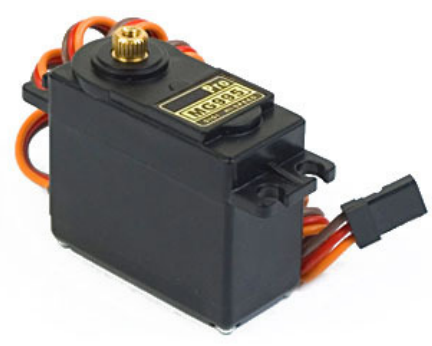
\includegraphics[scale  = 0.50]{Imagenes/servo_motor.png}
	\caption{Servo motor MG995}{Fuente: Adaptado de~\cite{servo_motor}}
\end{figure}

\begin{figure}[htb]
	\centering
	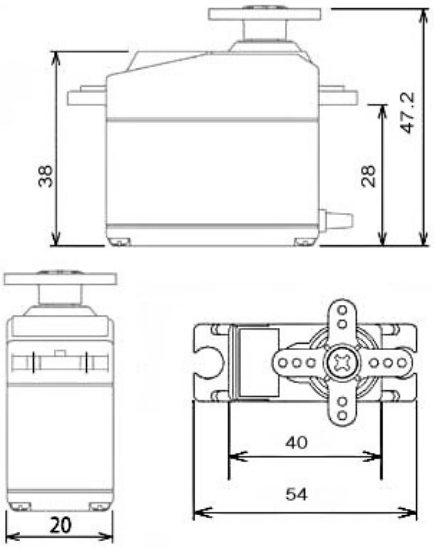
\includegraphics[scale  = 0.50]{Imagenes/dimensiones_servo.png}
	\caption{Dimensiones del servo motor}{Fuente: Adaptado de~\cite{servo_motor}}
\end{figure}

\begin{figure}[htb]
	\centering
	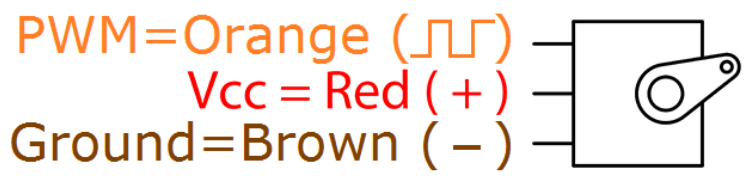
\includegraphics[scale  = 0.50]{Imagenes/cables_servo.png}
	\caption{Distribución de cables}{Fuente: Adaptado de~\cite{servo_motor}}
\end{figure}

\begin{figure}[htb]
	\centering
	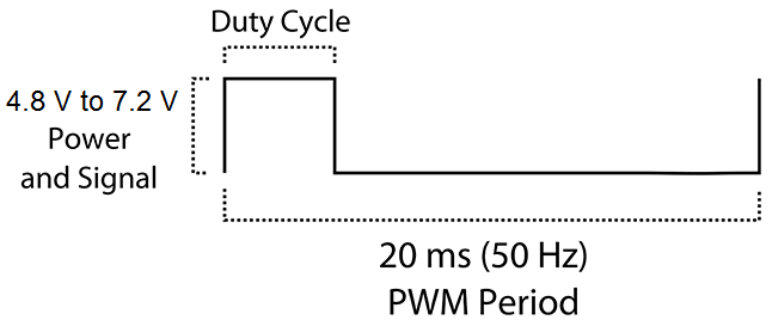
\includegraphics[scale  = 0.50]{Imagenes/consumo_servo.png}
	\caption{Consumo de energía}{Fuente: Adaptado de~\cite{servo_motor}}
\end{figure}

A continuación, se muestran las características técnicas extraidas del DataSheet encontrado:

\begin{table}[H]
    \centering
    \begin{tabularx}{\textwidth}{|l|X|} % Usar X para columnas que se expanden
        \hline
        \textbf{Especificación} & \textbf{Descripción} \\ 
        \hline
        \textbf{Dimensiones} & 40.7 mm x 19.7 mm x 42.9 mm \\ 
        \hline
        \textbf{Peso} & 55 g \\ 
        \hline
        \textbf{Ángulo de rotación} & 120º (60º en cada dirección) \\ 
        \hline
        \textbf{Torque detenido} & 8.5 kgf*cm (4.8 V), 10 kgf*cm (6 V) \\ 
        \hline
        \textbf{Banda muerta} & 5 $\mu$s \\
        \hline
        \textbf{Largo del cable} & 31 cm \\
        \hline
        \textbf{Voltaje de operación} & 4.8 a 7.2 V \\ 
        \hline
        \textbf{Velocidad de operación} & 0.2 s/60º (4.8 V), 0.16 s/60º (6 V)\\ 
        \hline
        \textbf{Rango de temperatura} & 0 a 55 ºC  \\
        \hline
        \textbf{Conector} & Universal para la mayoría de los receptores de radio control \\ 
        \hline
        \textbf{Compatibilidad} & Compatible con tarjetas como Arduino y microcontroladores que funcionan a 5 V. \\ 
        \hline
    \end{tabularx}
    \caption{Especificaciones del MG995}{Fuente: Adaptado de~\cite{servo_motor}}
    \label{tab:especificaciones_mg995}
\end{table}

